% Full local evaluation; measured provenance is preserved in data/provenance.json.
\documentclass[letterpaper,10pt,conference]{ieeeconf}
\IEEEoverridecommandlockouts
\overrideIEEEmargins
\usepackage[T1]{fontenc}
\usepackage{mathptmx}
\usepackage{amsmath,amssymb}
\usepackage{graphicx}
\usepackage{booktabs}
\usepackage{array}
\usepackage{cite}
\usepackage{url}
\usepackage{tikz}
\usetikzlibrary{arrows.meta,positioning}
\pdfminorversion=4
\pdfinfo{/Title (ANCHOR: Asset-Informed Geometric Skills for Language-Conditioned Manipulation)
 /Author (Anonymous) /Subject (ICRA 2027 anonymous manuscript)}
% Generated from data/episodes.jsonl; do not edit manually.
\newif\ifRunComplete
\RunCompletetrue
\newif\ifAllFresh
\AllFreshfalse
\newcommand{\EpisodeCount}{400}
\newcommand{\SuccessCount}{347}
\newcommand{\SuccessRate}{86.8}
\newcommand{\FailureCount}{53}
\newcommand{\ControllerFalsePositive}{11}
\newcommand{\ControllerMissedSuccess}{35}
\newcommand{\DisagreementCount}{46}
\newcommand{\DisagreementRate}{11.5}
\newcommand{\FreshCount}{390}
\newcommand{\FreshSuccessCount}{337}
\newcommand{\ReusedCount}{10}
\newcommand{\FreshSuccessRate}{86.4}
\newcommand{\FreshMedianSeconds}{66.5}
\newcommand{\RunMinutes}{70.2}
\newcommand{\RuntimeExceptionCount}{0}
\newcommand{\PerfectTaskCount}{21}
\newcommand{\SpatialRate}{91.0}
\newcommand{\SpatialMeanSteps}{147.4}
\newcommand{\ObjectRate}{96.0}
\newcommand{\ObjectMeanSteps}{173.0}
\newcommand{\GoalRate}{88.0}
\newcommand{\GoalMeanSteps}{180.9}
\newcommand{\LongRate}{72.0}
\newcommand{\LongMeanSteps}{293.3}
\newcommand{\TopDrawerSuccess}{3}
\newcommand{\DrawerPickSuccess}{5}
\newcommand{\BottomDrawerSuccess}{6}
\newcommand{\MokaSuccess}{4}
\newcommand{\MicrowaveSuccess}{0}

% Generated from model_audit.json and published_comparisons.json; do not edit.
\newcommand{\NeuralParameters}{172,249,090}
\newcommand{\NeuralMillion}{172}
\newcommand{\NeuralBillion}{0.172}
\newcommand{\DetectorWeightMB}{689}
\newcommand{\SmolParameterRatio}{2.6}
\newcommand{\OpenVLAParameterRatio}{40.6}

% Generated from recorded rollout selections; do not edit.
\newcommand{\RolloutSuccessTask}{Object 00}
\newcommand{\RolloutSuccessInit}{00}
\newcommand{\RolloutSuccessInstruction}{pick up the alphabet soup and place it in the basket}
\newcommand{\RolloutSuccessSteps}{136}
\newcommand{\OverviewBeforeImage}{figures/recorded/object_task00_init00_frame000.png}
\newcommand{\OverviewAfterImage}{figures/recorded/object_task00_init00_frame045.png}
\newcommand{\RolloutFailureTask}{Goal 03}
\newcommand{\RolloutFailureInit}{00}
\newcommand{\RolloutFailureInstruction}{open the top drawer and put the bowl inside}
\newcommand{\RolloutFailureSteps}{272}
\newcommand{\RolloutFailurePhaseStart}{111}
\newcommand{\RolloutFailurePhaseSteps}{161}
\newcommand{\RolloutFailureUnusedSteps}{28}

\newcommand{\method}{ANCHOR}
\newcommand{\R}{\mathbb{R}}
\title{\LARGE\bf ANCHOR: Asset-Informed Geometric Skills\\
for Language-Conditioned Manipulation}
\author{Anonymous Authors}

% Place Fig. 1 in the title block so it appears on the first page.
% Keep the class's caption style and the original two-column text geometry.
\makeatletter
\newcommand{\overviewcaption}[1]{\def\@captype{figure}\caption{#1}}
\makeatother
\IEEEaftertitletext{%
\begin{minipage}{\textwidth}
\centering
\resizebox{\textwidth}{!}{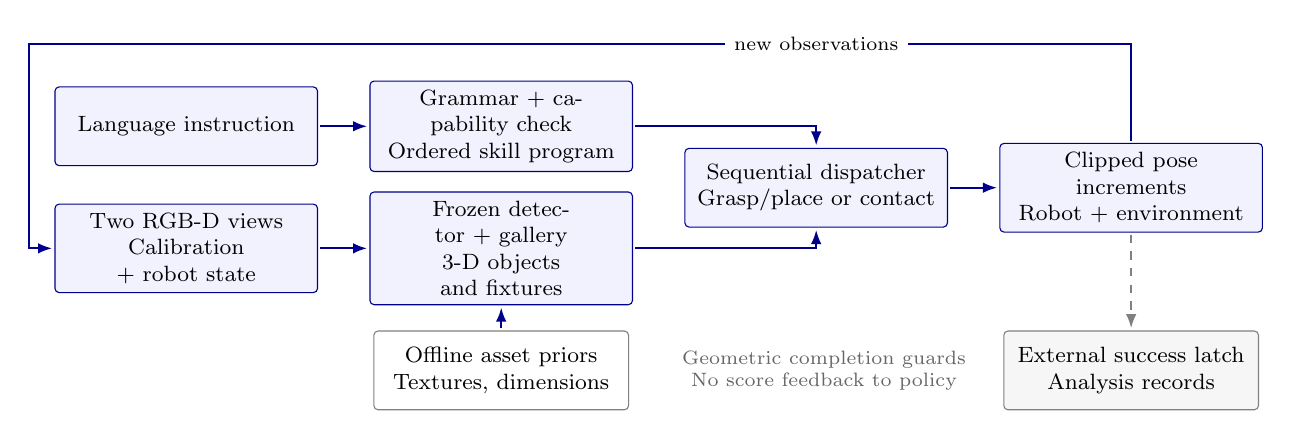
\begin{tikzpicture}[
    node distance=5mm and 8mm,
    box/.style={draw=blue!55!black, fill=blue!5, rounded corners=1.5pt,
      align=center, font=\footnotesize, minimum height=10mm, text width=31mm},
    smallbox/.style={box,text width=30mm,fill=white},
    flow/.style={-{Latex[length=1.8mm]}, thick, draw=blue!55!black},
    every node/.style={outer sep=1pt}
]
\node[box] (lang) at (0,1.55) {Language instruction};
\node[box] (compile) at (4.0,1.55) {Grammar + capability check\\Ordered skill program};
\node[box] (sensors) at (0,0) {Two RGB-D views\\Calibration + robot state};
\node[box] (perception) at (4.0,0) {Frozen detector + gallery\\3-D objects and fixtures};
\node[box] (control) at (8.0,.77) {Sequential dispatcher\\Grasp/place or contact};
\node[box] (robot) at (12.0,.77) {Clipped pose increments\\Robot + environment};
\node[smallbox,draw=gray] (prior) at (4.0,-1.55) {Offline asset priors\\Textures, dimensions};
\node[smallbox,draw=gray,fill=gray!7] (eval) at (12.0,-1.55) {External success latch\\Analysis records};
\draw[flow] (lang) -- (compile);
\draw[flow] (compile.east) -| (control.north);
\draw[flow] (sensors) -- (perception);
\draw[flow] (perception.east) -| (control.south);
\draw[flow] (prior) -- (perception);
\draw[flow] (control) -- (robot);
\draw[flow] (robot.north) -- (12,2.6) -- (-2.0,2.6) -- (-2.0,0) -- (sensors.west);
\node[font=\scriptsize,fill=white] at (8.0,2.6) {new observations};
\draw[-{Latex[length=1.8mm]},dashed,gray,thick] (robot) -- (eval);
\node[font=\scriptsize,align=center,text=gray!80!black] at (8.1,-1.55)
  {Geometric completion guards\\No score feedback to policy};
\end{tikzpicture}
}
\overviewcaption{From language to physical interaction with \method{}.
Supported instructions specify a skill sequence; calibrated RGB-D and asset
priors provide the geometry used to execute it. The controller carries object
and fixture state across stages and advances using local observation checks.
The frozen \NeuralMillion{}M-parameter detector is the only neural model.
Insets show the recorded \RolloutSuccessTask{} rollout; the geometry illustration is schematic.
External benchmark success is recorded separately from policy execution.}
\label{fig:architecture}
\vspace{3mm}
\end{minipage}%
}

\begin{document}
\bstctlcite{reference_style}
\maketitle
\thispagestyle{empty}
\pagestyle{empty}

\begin{abstract}
Multi-stage manipulation requires each skill to leave geometry and contact
conditions that the next skill can use. We present \method{}, an
asset-informed system that carries accepted scene estimates, grasp-dependent
object offsets, and fixture anchors between geometric skills. A deterministic
compiler maps supported instructions to a skill sequence, while local checks
on robot measurements and selected visual updates govern execution.
One frozen \NeuralMillion{}M-parameter detector, two calibrated RGB-D views,
and public asset priors supply the perceptual inputs. Manually designed
controllers generate actions without robot-demonstration training.
In a full evaluation of 400 fixed initializations spanning 40 LIBERO tasks,
one frozen controller reaches the official success predicate in
\SuccessCount{} episodes (\SuccessRate{}\%). Separate controller and evaluator
outcomes disagree in \DisagreementCount/\EpisodeCount{} episodes, exposing
limitations of local completion checks. The study characterizes geometric
execution under known-asset and calibrated-sensing assumptions.
\end{abstract}

\section{Introduction}
Consider the instruction to place a mug inside a microwave and close it.
The mug must enter the cavity in its grasped configuration, separate from the
fingers on release, and remain inside as the hand withdraws and engages the
door. A correct object label and skill sequence leave these physical
transitions unresolved. A mug caught on a finger can be pulled out by retreat;
a drawer opened successfully can leave the arm poorly configured for the
next grasp. Multi-stage execution therefore depends on both the goal of each
skill and the state it leaves for the next one.

Existing approaches connect language to action through several interfaces.
Vision-language-action (VLA) models learn action prediction from robot
demonstrations~\cite{openvla,smolvla,openvlaoft}. Program-based systems expose
perception and control calls~\cite{codepolicies}, while geometric approaches
express desired behavior through spatial value maps or keypoint
constraints~\cite{voxposer,rekep}. We study the execution interface in a
constrained setting with known assets, supported language forms, and
calibrated sensing. The question is how to connect perceptual estimates to
the geometric targets and transition checks needed across successive skills,
and how those explicit quantities help diagnose observed failures.

We present \method{} (Fig.~\ref{fig:architecture}), a language-conditioned
tabletop manipulation system built around three kinds of execution state.
Observed surfaces and asset dimensions determine contact and placement
regions. A carried-object offset converts an object goal into an end-effector
target. Local checks on pose, gripper width, visual geometry, and contact
evidence govern progression between stages. A deterministic compiler supplies
the skill sequence, while a frozen \NeuralMillion{}M-parameter Grounding DINO
detector and an asset gallery ground objects in two calibrated RGB-D views.
The system generates actions through manually designed controllers, with no
robot-demonstration training of an action policy.

We evaluate 40 tasks from LIBERO's Spatial, Object, Goal, and Long
suites~\cite{libero}, with ten official initial states per task and one frozen
controller. This system study contributes:

\begin{enumerate}
\item An asset-informed execution interface that connects accepted scene
      estimates, grasp-dependent offsets, and fixture anchors to the targets
      and transition checks of manipulation skills.
\item A complete evaluation on 40 tasks, with declared sensing and prior
      knowledge, an audited neural model count, and reproducible episode records.
\item An analysis of phase traces, failure locations, and stopping outcomes
      that identifies mismatches between local completion and the benchmark
      predicate in the evaluated controller.
\end{enumerate}

\section{Related Work}
\subsection{Geometric Representations for Manipulation}
Task and motion planning couples discrete action choices with continuous
geometric feasibility~\cite{tamp}. kPAM uses
semantic 3-D keypoints to specify manipulation goals as geometric costs and
constraints~\cite{kpam}. VoxPoser grounds language in spatial value maps for
motion planning~\cite{voxposer}, and ReKep optimizes sequences of relational
keypoint constraints~\cite{rekep}. \method{} shares the use of explicit geometry
between perception and action. Its representation consists of object bounds,
support and fixture geometry, and carried-object offsets, consumed by
specialized finite-state skills. This fixed skill structure defines its
coverage; it does not optimize a general task-and-motion problem.

\subsection{Language and Executable Skills}
SayCan combines language-model proposals with learned skill affordances to
select executable actions~\cite{saycan}. Code as Policies generates programs
that process perceptual outputs, express control logic, and call robot
interfaces~\cite{codepolicies}. These systems use language models to construct
behavior. \method{} binds spatial references to observed entities using a
deterministic grammar and a checked skill vocabulary. The grammar fixes
language coverage; our study concerns execution and the state passed between
its skills.

\subsection{Pretrained Perception and Learned Action Policies}
Grounding DINO provides text-conditioned object proposals~\cite{groundingdino}.
\method{} combines its frozen detector with calibrated depth and asset-derived
texture and size priors. OpenVLA~\cite{openvla} and SmolVLA~\cite{smolvla}
learn robot action generation from demonstrations, with SmolVLA
emphasizing a compact architecture. OpenVLA-OFT studies design choices for
faster and more successful VLA execution~\cite{openvlaoft}.
Section~\ref{sec:comparison} compares their model requirements and reported
outcomes with \method{}, accounting for its asset knowledge and manual
skill development.

\section{Method}
\label{sec:method}
\method{} compiles an instruction, grounds its entities, and executes the
resulting skills in order (Fig.~\ref{fig:architecture}). Each phase constructs
a pose and gripper target from the available geometry and uses local
checks to continue, advance, retry, or terminate. Table~\ref{tab:conditions}
declares the available information; Table~\ref{tab:state} describes the
state passed through this execution interface.

\subsection{Task and Information Interface}
Given an instruction $\ell$, the controller produces actions
$a_t=\pi(o_{\leq t},\ell;\mathcal{P})$, where $\mathcal{P}$ contains fixed
prior information and the observation at step $t$ is
\begin{equation}
 o_t=\left(\{I_t^c,D_t^c,K^c,T_{WC,t}^c\}_{c\in\{a,w\}},r_t\right).
\end{equation}
Here $a$ and $w$ denote the fixed and wrist cameras, $I$ is RGB,
$D$ is metric depth, $K$ is calibration, and $T_{WC}$ maps camera
coordinates into the world frame. Robot measurements $r_t$ include
end-effector pose, joint state, gripper state, and available force/torque
measurements. The grasp--place adapter uses pose, joint positions, and gripper
width; contact execution can access the broader robot measurement interface.

Depth, camera calibration, and robot measurements are supplied by the
simulator adapter. The policy observation types exclude object pose labels,
segmentation IDs, BDDL predicates, reward, and task-success flags. Task
identifiers and initial-state indices remain with the evaluator; reset passes
the instruction and a nonsemantic episode token.

The prior collection $\mathcal{P}$ contains object texture histograms,
dimensions derived from public collision geometry, robot geometry,
class-specific handling rules, and motion thresholds. These priors specify
how to interpret observations and parameterize skills. The neural detector
is pretrained; the action controller is designed manually. No action-policy
fitting or robot-demonstration loading occurs in the evaluation.

\begin{table}[t]
\caption{Declared conditions for the evaluated system.}
\label{tab:conditions}
\centering
\footnotesize
\begin{tabular}{@{}p{.32\columnwidth}p{.63\columnwidth}@{}}
\toprule
Property & Setting \\
\midrule
Policy observations & Fixed and wrist RGB-D, camera calibration, robot measurements \\
Offline priors & Public asset textures/dimensions, robot geometry, hand-written skill rules \\
Action generation & Geometric state machines and clipped Cartesian increments \\
Neural model & One frozen Grounding DINO Tiny (\NeuralMillion{}M parameters) \\
Action-policy training & None; skills and thresholds are designed manually \\
Scene truth in policy & No object pose labels, segmentation IDs, or BDDL predicates in observation types \\
Success feedback & External latch; no score-driven policy stopping \\
Coverage & Known benchmark assets and implemented instruction grammar \\
\bottomrule
\end{tabular}
\end{table}

\subsection{Constrained Language Compilation}
The compiler maps supported language to
\begin{equation}
 \mathcal{G}(\ell)=(s_1,\ldots,s_M),\qquad
 s_j=(k_j,e_j^{\rm src},e_j^{\rm dst},\rho_j).
\end{equation}
Here $k_j$ is a skill, the entity bindings specify source and destination,
and $\rho_j$ represents a placement relation or instance selector.
The vocabulary contains pick, place-on, place-in, relative placement,
stack, open, close, push, turn-on, and turn-off. For example, opening a
drawer and placing a bowl inside produces an articulation segment followed
by pick and place-in steps. A two-object basket instruction produces two
successive pick/place pairs.

Bindings retain relations such as \emph{next to}, \emph{between}, or an
ordering among visible instances. They do not encode simulator object
identity. Before motion, the compiler checks skill arguments and held-object
consistency, including whether each place step refers to the object acquired
by a preceding pick. Physical executability is assessed during skill
execution. The grammar covers known LIBERO phrases and an allow-listed entity
vocabulary; no language-model resolver is configured.

\subsection{State across Skill Boundaries}
The execution state links the current skill and phase to accepted scene
geometry, a carried-object offset, and fixture anchors
(Table~\ref{tab:state}). Robot pose and gripper measurements support the
servo at every action step. Visual grounding is invoked at selected stages;
observing a new frame does not imply re-estimating every target. Some refresh
routines compare new estimates with the stored geometry to reject changes
caused by hand occlusion.

This persistence matters across interactions. Placement consumes the offset
established by the grasp; a placement after drawer opening consumes its
observed drawer anchor; sequential stove placements share a support estimate
obtained while the burner is unoccluded. The stored quantities make these
dependencies explicit, while their update rules determine when new evidence
can revise a target.

\begin{table}[t]
\caption{Geometric state and its use during execution. Updates are selected
by the active skill and phase.}
\label{tab:state}
\centering
\footnotesize
\begin{tabular}{@{}>{\raggedright\arraybackslash}p{.22\columnwidth}@{\hspace{5pt}}>{\raggedright\arraybackslash}p{.36\columnwidth}@{\hspace{5pt}}>{\raggedright\arraybackslash}p{.36\columnwidth}@{}}
\toprule
State & Source or update & Use \\
\midrule
Scene estimates & RGB-D grounding with texture and size priors & Entity binding, approach and placement regions \\
Carried offset $\hat d_t$ & Grasp geometry; selected RGB-D refreshes & Object goal to end-effector target, Eq.~\eqref{eq:offset} \\
Fixture anchors & Visible support/fixture fits and contact-skill outputs & Subsequent placement and fixture interaction \\
Phase and counters & Local checks and executed actions & Advancement, bounded recovery, stopping \\
\bottomrule
\end{tabular}
\end{table}

\subsection{Asset-Informed Visual Grounding}
The deployed Grounding DINO Tiny checkpoint contains
\NeuralParameters{} unique parameters, including its visual and text
encoders. All weights are frozen, and one detector instance serves both
camera views in each evaluation process. The asset gallery, language
compiler, and geometric controllers add no neural model parameters.
The pinned checkpoint and parameter audit are included in the manuscript
artifacts.

Each calibrated pixel $\tilde u=(u,v,1)^\top$ with valid depth contributes
\begin{equation}
 x_W=R_{WC}\big(D(u,v)K^{-1}\tilde u\big)+p_{WC}.
 \label{eq:backproject}
\end{equation}
Here $R_{WC}$ and $p_{WC}$ are the rotation and translation of $T_{WC}$.
Workspace filtering, support estimation, and connected components produce
candidate point sets. Grounding DINO supplies additional language-conditioned
boxes, which are converted to 3-D hypotheses using depth. These proposals
are combined with observed bounds and asset-derived texture and size
evidence. The gallery compares normalized HSV histograms using
\begin{equation}
 b(h,h_k)=\sum_i\sqrt{h_i h_{k,i}}.
\end{equation}
Its classification score combines color and shape terms,
with configured weights $0.4$ and $0.6$, a softmax temperature of $0.13$,
and additional class-dependent footprint gates. This combination associates
visual proposals with known asset classes without an oracle object mask.

Cross-camera hypotheses with matching labels are clustered in 3-D. For a
cluster, the implemented fusion weights are proportional to
$\max(q_i,0.05)\sqrt{n_i}$, where $q_i$ is confidence and $n_i$ is point
count. The default center-distance threshold is $4.5$\,cm.
The resulting state distinguishes observed bounds and supports from geometry
completed using size priors. A prior can stabilize the center of a partly
visible object without establishing that an unobserved region is free.

Geometric selectors bind instruction references to candidate instances.
At selected phase transitions, fresh views are checked against previous
estimates to reject abrupt changes caused by hand occlusion. Nearby repeated
objects can still produce ambiguous associations. Fixture routines further
refine the selected geometry into support surfaces and opening regions.

\subsection{Carried-Object Geometry and Placement}
\label{sec:placement}
Consecutive manipulation skills share a grasp--place controller. Its phases
include acquisition, pregrasp motion, approach, finger closure, retention
checking, lift, transport, descent, release, and retreat. Transitions combine
pose tolerances, measured gripper width, visual evidence, and bounded retry
logic. The evaluated configuration uses exterior pinch and closing rim
pinches. Object-class rules select the nominal mode; observed geometry
determines the grasp target and available retries.

The chosen grasp also determines the geometry used during placement.
In particular, the gripper and carried object generally have different
centers. Let $\hat d_t$ be the estimated world-frame vector from the end
effector to the carried-object reference point. For desired object location
$p_o^\star$, placement uses
\begin{equation}
 p_{\rm ee}^\star=p_o^\star-\hat d^\star,\qquad
 \hat d^\star=\Delta R\,\hat d_t.
 \label{eq:offset}
\end{equation}
Here $\Delta R=R_{\rm ee}^\star R_{{\rm ee},t}^{\top}$ is the planned wrist
rotation in the world frame. The relation assumes that the object remains
fixed relative to the gripper over this motion; slip or partial release can
invalidate that estimate. The implementation supplements Eq.~\eqref{eq:offset}
with support, release-height, aperture, and fixture-specific corrections.
The offset is estimated from precontact geometry or refreshed RGB-D evidence;
its origin is retained in the execution trace.

Placement must also leave room for the hand to withdraw. Microwave entry
aligns the carried object with the cavity width and uses a lateral approach.
Repeated basket placements use separate diagonal landing centers. Before
basket withdrawal, the controller checks measured jaw clearance and can
apply a bounded wrist tilt to clear a tall object near the palm. Release is
followed by a geometric observation check before the program advances.

For microwave release, retreat waits for a measured 78-mm jaw opening and
a settling dwell, because a commanded opening alone does not establish
that the mug rim has cleared the fingers.

\subsection{Fixture Geometry and Contact Skills}
The dispatcher separates consecutive grasp--place steps from atomic contact
skills. Drawer and door interactions use observed fixture geometry to
construct approach, engagement, motion, release, and retreat stages.
Knob and push skills use their own target detectors and motion templates.
Shared episode state includes an initial robot-pose reference and, where
applicable, an observed drawer anchor for subsequent placement.

Grounded object boxes are refined into surfaces needed for physical
interaction. A complete visible burner disk anchors the stove support center;
public plate thickness supplies the offset to the load-bearing surface.
That unoccluded estimate is retained across sequential placements. For an
open microwave, visible vertical control-panel and side-wall surfaces,
together with the roof height, constrain the cavity and hinge frame through
public physical dimensions. A flat tabletop crop or a roof without supporting
vertical structure is insufficient for this fit.

For microwave closure, the skill fits a vertical door panel within the
observed hinge sweep. Initial fitting requires panel evidence outside the
appliance body to exclude the fixed front frame. The gripper approaches
the exterior panel face and follows bounded hinge-frame waypoints.
A fresh angle estimate after a motion plateau can initiate withdrawal;
a second view after retreat checks closure.

After drawer contact, the next grasp may require substantial wrist motion.
The controller compares equivalent jaw frames along a continuous
inverse-kinematics path using the public robot model and bounds simultaneous
translation and rotation. This is a local reachability heuristic, without
collision checking. During bowl transport, it uses the observed drawer front
and held-object footprint to move clear of the panel before lifting.

Contact guards combine position error, measured progress, and changes in
end-effector force. One guard requires a minimum contact duration and bounded
position error, plus either stalled error reduction or sufficient force
change. This provides evidence of contact; a subsequent visual check assesses
the resulting fixture configuration. The separation allows the controller
to distinguish a mechanical stop from its estimate of task completion.

\subsection{Action Generation and Transition Checks}
For a geometric target pose $(p^\star,R^\star)$ and gripper command $g_t$,
the basic Cartesian servo emits
\begin{equation}
 a_t=\operatorname{clip}_{[-1,1]}
 \begin{bmatrix}
 (p^\star-p_t)/s_p\\
 \operatorname{Log}(R^\star R_t^\top)^\vee/s_R\\
 g_t
 \end{bmatrix}.
 \label{eq:servo}
\end{equation}
The rotation term is the axis-angle error between the current and target
orientations.
The general grasp--place scales are $s_p=0.05$\,m and
$s_R=0.25$\,rad; cavity handling can select another rotation scale.
Nominal pose tolerances of $8$\,mm and $0.12$\,rad gate transitions between
motion phases. Specialized branches additionally bound translation or
rotation during constrained motions.

Phase counters and geometric checks bound local recovery. The controller may
release a rejected grasp, reacquire a visible handle, or execute a short
clearance motion after stalled drawer interaction. Each stage supplies
explicit targets, observations, and stopping reasons for inspection. These
checks govern execution using the policy's own measurements. The benchmark
predicate is unavailable to both action selection and stopping, so local
completion remains a separate outcome, evaluated in
Section~\ref{sec:outcomes}.

\section{Experimental Protocol}
\label{sec:protocol}
\subsection{Tasks, Initial States, and Runtime}
The evaluation contains $4\times10\times10=400$ episodes:
Spatial, Object, Goal, and Long, ten tasks each, and official initial-state
indices $0$--$9$. Long is named \texttt{libero\_10} in the implementation.
Global random generators and the environment configuration use seed $7$.
The environment adapter preserves or replays the task reset stream when
starting at a later initial-state index, because resetting can affect fixture
configuration beyond the saved joint state.

We use two $256\times256$ RGB-D cameras and a Panda with operational-space
pose control. A ten-step settling period precedes scored actions. The
Spatial/Object/Goal/Long action budgets are $220/280/300/520$, matching
the numerical budgets in the OpenVLA evaluation script~\cite{openvlacode}.
Our environment seed and success-handling logic differ from that script;
its environment utility uses seed $0$.
The full run uses Ubuntu 24.04 under WSL2, Python 3.12.14,
PyTorch 2.11.0 with CUDA 13.0, MuJoCo 3.3.2~\cite{mujoco},
robosuite 1.4.0~\cite{robosuite}, and hf-libero 0.1.4 on one RTX 3090.

All 400 episodes are newly executed against one immutable source snapshot.
Independent task processes run under a dispatcher, initially with four
workers and then six. Each process starts from the declared seed and evaluates
the ten initializations of one task in index order. Before evaluation, all
simulator assets and model files are checked against pinned SHA256 hashes.
The source manifest, effective configuration, episode coverage, and scoring
mode are validated after the full run. The task initializations include
states used during skill development; this evaluation does not measure
held-out generalization.

\subsection{External Scoring and Internal Completion}
Let $q_t$ be the official success predicate observed by the evaluator.
With policy-controlled stopping time $\tau$ capped at budget $H$, the
recorded outcome is
\begin{equation}
 Y=\bigvee_{t=1}^{\tau}q_t\ \lor\ q_{\rm final},
 \qquad \tau\leq H.
 \label{eq:score}
\end{equation}
The final query also handles a zero-action stop. Reward and success do not
enter the policy observation. The evaluator continues after a success signal
until the controller requests stopping or the action budget expires.
The score therefore represents \emph{ever reaching} the predicate during
this rollout, not necessarily satisfying it at the final frame.

Each record additionally stores terminal controller state, step count,
elapsed time, failure message, and geometric traces. The reported success rate
is $\widehat p=N^{-1}\sum_iY_i$. Equal task sample counts make the overall
episode average equal to the macro-average over tasks in the completed run.
All planned episodes, including unsuccessful rollouts, enter the reported
statistics. Controller-internal retries remain within one episode.

\subsection{Scope of the Evidence}

The completed campaign passes its record-coverage validation: 400 unique
episodes, fixed configuration, existing recorded videos, and matching
deployed source checksums.

Tables are generated from hashed original records. Published values are
stored separately with their cited sources. Per-task counts expose the
sample size behind each rate.

\begin{table}[t]
\caption{External ever-success counts and execution cost.
$^\dagger$Elapsed-time medians include execution overhead under concurrent
evaluation. All counts, steps, and times come from the same full run.
}
\label{tab:results}
\centering
\footnotesize
\begin{tabular}{lrrrr}
\toprule
Suite & Success & SR (\%) & Mean steps & Median s$^\dagger$ \\
\midrule
Spatial & 91/100 & 91.0 & 147.4 & 68.7 \\
Object & 96/100 & 96.0 & 173.0 & 54.7 \\
Goal & 88/100 & 88.0 & 180.9 & 67.2 \\
Long & 72/100 & 72.0 & 293.3 & 90.4 \\
\midrule
Overall & 347/400 & 86.8 & 198.6 & 66.5 \\
\bottomrule
\end{tabular}

\end{table}

\section{Results and Analysis}
\subsection{Task Outcomes}

The frozen system records \SuccessCount{} successes in 400 episodes
(\SuccessRate{}\%; Table~\ref{tab:results}).

The suite rates are
\SpatialRate{}\% for Spatial, \ObjectRate{}\% for
Object, \GoalRate{}\% for Goal, and \LongRate{}\% for Long.
Long contains \LongFailureCount{} of the \FailureCount{} external failures
(\LongFailureShare{}\%), despite contributing one quarter of the episodes.
The overall rate therefore masks lower reliability on the Long suite.

The task distribution reveals variation hidden by the overall rate
(Fig.~\ref{fig:tasks}). \PerfectTaskCount{} tasks have ten successful recorded
trials. Long 09, placing a mug inside a microwave and closing it, records
$\MicrowaveSuccess/10$; Long 08, placing both moka pots on the stove, records
$\MokaSuccess/10$. These tasks require confined access, sequential placement,
or fixture interaction. Drawer-related tasks also differ: Goal 03, opening
the top drawer and placing a bowl inside, records $\TopDrawerSuccess/10$;
Spatial 04, retrieving a bowl from a top drawer, records
$\DrawerPickSuccess/10$; and Long 03, placing a bowl in a bottom drawer and
closing it, records $\BottomDrawerSuccess/10$. The variation motivates
examining individual execution stages rather than attributing all failures
to a task category.

\begin{figure*}[t]
\centering
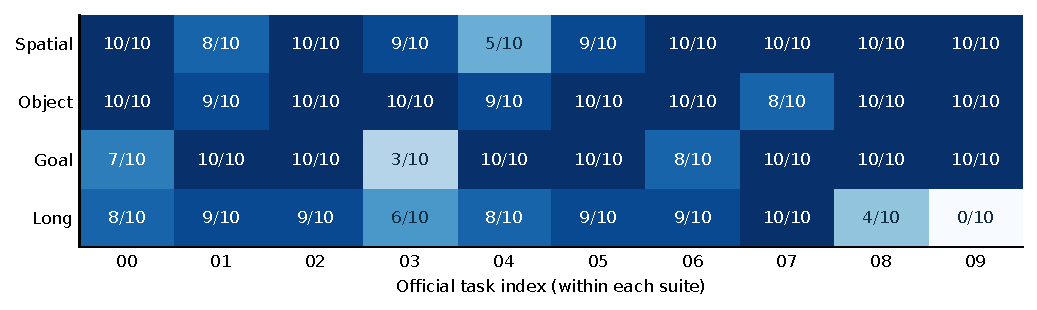
\includegraphics[width=\textwidth]{figures/per_task.pdf}
\caption{External successes per ten trials. Columns identify different tasks
in each suite; darker cells indicate higher success.
}
\label{fig:tasks}
\end{figure*}

\subsection{Execution Traces and Visual Examples}
Figure~\ref{fig:rollouts} aligns recorded images with the executed action
count and logged control phase. These labels expose which stage produced
the motion, while the underlying traces retain its geometric targets and
accepted observations.

The successful \RolloutSuccessTask{} example completes in
\RolloutSuccessSteps{} actions. In the \RolloutFailureTask{} example, the
controller enters pregrasp at action count \RolloutFailurePhaseStart{} and
remains in that phase for \RolloutFailurePhaseSteps{} actions before stopping
at \RolloutFailureSteps{}, with \RolloutFailureUnusedSteps{} actions left in
the episode budget. The timeout locates the unsuccessful stage after drawer
interaction; it does not establish whether contact, an unreachable target,
or estimation error caused the stall.

\subsection{Local Completion and External Success}
\label{sec:outcomes}
Table~\ref{tab:status} crosses local completion with external ever-success.
Of \ControllerCompleteCount{} locally completed episodes,
\CompletedExternalSuccessCount{} reach the official predicate
(\CompletionAgreementRate{}\%), while \ControllerFalsePositive{} never do.
Conversely, \ControllerMissedSuccess{} episodes reach external success
without controller completion. The total disagreement is
\DisagreementCount{}/\EpisodeCount{} (\DisagreementRate{}\%).

Local checks can therefore accept a rollout that never satisfies the goal,
or continue demanding a geometric relation after the goal has been reached.
The latter group includes later local failures and global-budget timeouts.
This cross-tabulation exposes the scope of local verification: an
ever-success label does not establish that the controller recognizes or
preserves the goal until stopping.

The records retain neither first-success time nor a separate final-state
label. They therefore cannot determine how continued execution changes
final-state success or how much runtime an early-stop evaluator would save.

\begin{table}[t]
\caption{Terminal controller state and independently recorded external
ever-success.
A controller failure can follow an earlier benchmark success.}
\label{tab:status}
\centering
\footnotesize
\begin{tabular}{lrr}
\toprule
Controller terminal state & External success & External failure \\
\midrule
Succeeded & 341 & 6 \\
Failed & 24 & 18 \\
Timeout & 11 & 0 \\
\bottomrule
\end{tabular}

\end{table}

\subsection{Remaining Failure Categories}
Table~\ref{tab:failures} groups all \FailureCount{} external failures by
terminal state and message. Phase timeouts form the largest group.
Grouping prioritizes controller completion with external failure and global
budget exhaustion before classifying the remaining termination messages.
All \EarlyFailureCount{} externally unsuccessful episodes stop before their
global action cap, leaving at least \FailureMinUnusedSteps{} actions unused.
Conversely, all \GlobalTimeoutCount{} global-budget timeouts have an external
success label. The observed external failures therefore end at local stopping
conditions, which motivates examining phase targets and termination checks.

These categories locate where execution stopped. They do not identify
physical root causes: a timeout can arise from an inaccessible target,
occlusion, calibration error, or contact resistance, and a rejected
verification can reflect either placement error or uncertain perception.
Per-episode geometric traces and recordings supply the additional evidence
needed to investigate a particular failure.

\begin{table}[t]
\caption{Outcome groups among external failures. Categories are derived from recorded controller
messages with a fixed precedence rule.}
\label{tab:failures}
\centering
\scriptsize
\begin{tabular}{lr}
\toprule
Recorded outcome group & Episodes \\
\midrule
Phase timeout & 15 \\
Controller completion / external failure & 7 \\
Global action budget & 4 \\
Grasp / retention rejection & 3 \\
Other controller failure & 2 \\
Sensor verification rejection & 1 \\
\bottomrule
\end{tabular}

\end{table}

\begin{figure*}[t]
\centering
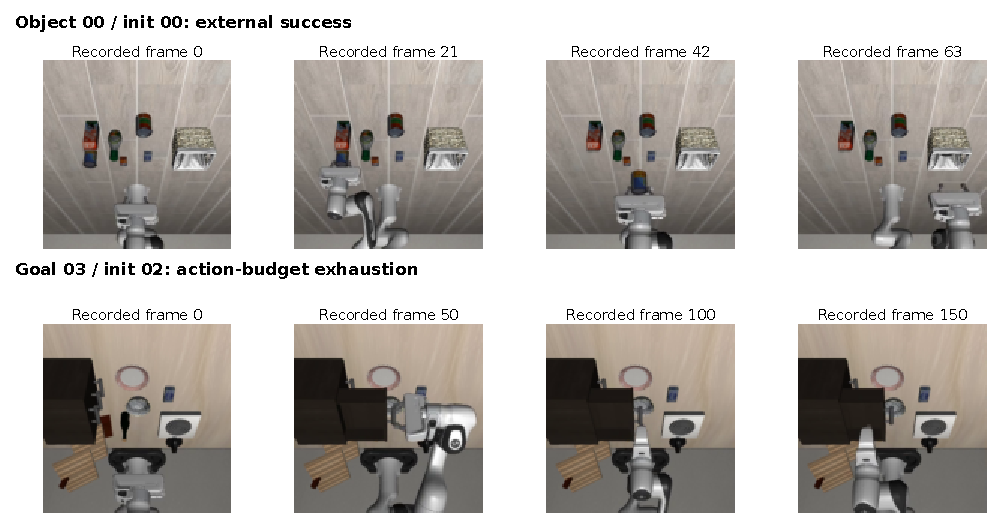
\includegraphics[width=.90\textwidth]{figures/rollouts.pdf}
\caption{Actual fixed-camera frames from the local full evaluation. Top:
\emph{\RolloutSuccessInstruction} (\RolloutSuccessTask,
initial state \RolloutSuccessInit). Bottom: \emph{\RolloutFailureInstruction}
(\RolloutFailureTask, initial state \RolloutFailureInit).
Four uniformly spaced frames are shown. $t$ counts executed actions, and
phase labels use the last logged transition at or before $t$. The bottom
bar shows the failed episode's earlier actions, final active phase, and
unused global budget. Frames are vertically flipped for upright display;
left/right is preserved.}
\label{fig:rollouts}
\end{figure*}

\begin{table}[t]
\caption{Model size and robot-demonstration use for action-policy training.
VLA sizes are rounded values from the cited papers; \method{} counts all
unique parameters in its deployed detector. ``None'' refers to action-policy
training, not to perception pretraining or manual skill development.}
\label{tab:models}
\centering
\footnotesize
% Generated from model_audit.json and published_comparisons.json; do not edit.
\begin{tabular*}{\columnwidth}{@{\extracolsep{\fill}}lrc@{}}
\toprule
Method & Parameters & Policy training \\
\midrule
SmolVLA~\cite{smolvla} & 0.45B & Robot demos \\
OpenVLA~\cite{openvla} & 7B & Robot demos \\
OpenVLA-OFT~\cite{openvlaoft} & 7B & Robot demos \\
\midrule
\method{} & \NeuralBillion{}B & None \\
\bottomrule
\end{tabular*}

\end{table}

\begin{table*}[t]
\caption{LIBERO success rates (\%). Published rows contain the reported
means from OpenVLA v3, Table~12~\cite{openvla}, SmolVLA v1,
Table~2~\cite{smolvla}, and OpenVLA-OFT v2, Table~I~\cite{openvlaoft}
(arXiv versions); they are not reruns by us.
OpenVLA-OFT uses its full setting.
The final row is measured in this work.
All methods receive language; their sensing, training, and protocols differ.}
\label{tab:published}
\centering
\footnotesize
% Generated from published_comparisons.json and episodes.jsonl; do not edit.
\begin{tabular*}{\textwidth}{@{\extracolsep{\fill}}lp{.36\textwidth}rrrrr@{}}
\toprule
Method & Sensing and action-policy setup & Spatial & Object & Goal & Long & Average \\
\midrule
\multicolumn{7}{@{}l}{\emph{Published results (reported means)}} \\
Diffusion Policy~\cite{openvla} & Single RGB; policy trained from scratch per suite & 78.3 & 92.5 & 68.3 & 50.5 & 72.4 \\
Octo~\cite{openvla} & Single RGB; pretrained policy fine-tuned per suite & 78.9 & 85.7 & 84.6 & 51.1 & 75.1 \\
OpenVLA~\cite{openvla} & Single RGB; pretrained policy fine-tuned per suite & 84.7 & 88.4 & 79.2 & 53.7 & 76.5 \\
SmolVLA (0.45B)~\cite{smolvla} & RGB/state; VLM-initialized policy trained across suites & 90.0 & 96.0 & 92.0 & 71.0 & 87.3 \\
OpenVLA-OFT~\cite{openvlaoft} & Two RGB views + state; policy fine-tuned per suite & 97.6 & 98.4 & 97.9 & 94.5 & 97.1 \\
\midrule
\multicolumn{7}{@{}l}{\emph{Measured in this work}} \\
\method{} & Two RGB-D views + state; asset priors, geometric skills & 93.0 & 98.0 & 97.0 & 86.0 & 93.5 \\
\bottomrule
\end{tabular*}

\end{table*}

\subsection{Model Requirements and Published Results}
\label{sec:comparison}
Table~\ref{tab:models} separates neural model size from the use of robot
demonstrations for action generation. \method{} has \NeuralBillion{}B
parameters in its frozen detector and no learned action network. The FP32
weight file occupies \DetectorWeightMB{}\,MB (decimal). The reported
SmolVLA and 7B OpenVLA model classes have approximately \SmolParameterRatio{}
and \OpenVLAParameterRatio{} times as many parameters, respectively.
Our count includes both visual and text encoders; the VLA sizes are rounded
descriptions from the source papers.

The selected SmolVLA simulation model starts from a VLM without robotics
pretraining but trains its action policy on LIBERO demonstrations~\cite{smolvla}.
\method{} relies on pretrained perception, asset priors, and manual skill
development; its parameter count quantifies only the neural component.



Table~\ref{tab:published} provides literature context for these requirements.
External rows retain the source papers' reported LIBERO means and averages;
\method{} is the only system evaluated in this study.

The OpenVLA study uses filtered demonstrations and reports averages over
three random seeds, with 500 trials per suite and seed~\cite{openvla}.
SmolVLA trains across all 40 tasks and evaluates ten trials per
task~\cite{smolvla}; OpenVLA-OFT uses filtered demonstrations and evaluates
500 trials per suite in the selected setting~\cite{openvlaoft}.
Our system uses calibrated RGB-D, public asset priors, ten official
initializations per task, and the ever-success rule in Eq.~\eqref{eq:score}.

The comparison describes different allocations of prior knowledge:
learned action policies use robot demonstrations, while \method{} uses
calibrated geometry and manually designed skills. These sensing, training,
and protocol differences preclude attributing differences in success rate
to the action representation or neural model size. Parameter counts also
provide no measurement of relative latency or peak memory.

\subsection{Execution Cost}
Long episodes use \LongMeanSteps{} actions on average, compared with
\ObjectMeanSteps{} for Object (Table~\ref{tab:results}). These counts extend
to the controller's stopping condition or the budget, so they measure the
cost of executed behavior rather than time to first success.

The median newly executed episode takes \FreshMedianSeconds{} seconds;
dispatcher wall time is \RunMinutes{} minutes.

The records contain \RuntimeExceptionCount{} runtime exceptions.
Elapsed times include perception, simulation, rendering, and video overhead
under the local hardware and concurrent scheduling. They describe
this evaluation environment and do not measure real-robot control frequency.

\section{Discussion and Limitations}
The evaluation characterizes geometric execution under explicit asset and
sensing assumptions. Stored targets, accepted geometry, and transition checks
make the controller's decisions available for inspection. The difference
between local completion and external success shows where this operational
interpretation of a task can diverge from the benchmark predicate. In this
run, external failures arise before the global action cap; the recorded phase
targets and stopping checks provide concrete locations for further study.

\paragraph{Prior knowledge and development effort}
The system's compact neural component relies on calibrated RGB-D,
public asset textures and dimensions, robot geometry, a constrained grammar,
and manually developed skills. Removing demonstration-based action-policy
training shifts work to these representations and procedures. Parameter
count and weight-file size quantify the detector, but do not quantify total
engineering cost, peak memory, or end-to-end latency. Debugging effort was
not compared with that of a learned policy.

\paragraph{Evaluation scope}
The study covers known assets and instruction forms in one simulated
embodiment. It does not test unseen assets, unrestricted language, perturbed
calibration, or physical hardware. LIBERO was introduced for lifelong robot
learning~\cite{libero}; the present evaluation characterizes manipulation
execution and does not measure transfer, continual learning, or forgetting.
The initializations include states used during skill development, so the
full run measures execution on the declared task set. No component ablations establish the
individual contribution of the gallery, offset handling, or local guards.
A fixed-controller evaluation on held-out conditions and ablations under
matched sensing would be needed to test robustness and separate those effects.

\paragraph{Execution and measurement limits}
Clipped commands, pose tolerances, and bounded retries are operational
controls, not guarantees of tracking accuracy, collision avoidance, or
contact safety. Small task samples can conceal rare failures, and the
observed disagreement between controller and evaluator shows why stopping
conventions matter. Recording first-success time and final-state success
separately would distinguish goal attainment from goal preservation.

\paragraph{Reproducibility}
The artifacts preserve original episode records, controller and resource
checksums, and table/figure generation scripts. Observation restrictions
are supported by interface and code inspection.

\section{Conclusion}
We presented \method{}, an asset-informed system that connects language
instructions to geometric manipulation skills through observed scene
geometry, carried-object offsets, and local transition checks. One frozen
\NeuralMillion{}M-parameter detector supplies its neural component, with
no robot-demonstration training of an action policy.

The complete evaluation records \SuccessCount/\EpisodeCount{} external
successes (\SuccessRate{}\%).

These results support inspectable geometric execution with known assets.
Generalization and the causal benefit of individual components require
further evaluation.

\section*{Acknowledgments and AI Disclosure}
OpenAI GPT-6-Astra (via Codex) assisted in drafting and editing the text in all sections,
preparing the LaTeX source, and writing scripts for the numerical tables and
figures. Results for \method{} are computed from existing simulator evaluation
records; comparison values are taken from the cited publications.
The rollout images are extracted from our recordings; no
generative image model was used.

\IEEEtriggeratref{8}
\bibliographystyle{IEEEtran}
\bibliography{references}
\end{document}
